\section{Splice Track II: A 2004 Baseline Beats Our CNN, and What Survives}
We compared the ClinVar-trained CNN against MaxEntScan \cite{yeo2004} on the same gene-grouped folds (n=9235 variants). MaxEntScan's ref$-$alt score difference reached AUROC 0.9635, above the CNN (0.9355), the logistic PWM model (0.9121) and the raw PWM delta (0.8893). The paired bootstrap 95\% CI for CNN minus MaxEntScan is [-0.0329, -0.0233], so this is a clear negative result for the CNN. The gap is mostly at acceptors (CNN 0.8794 vs MaxEntScan 0.965, n=3845); at donors the two are close (0.9538 vs 0.9598, n=5390).
As a pivot we added the three MaxEntScan features to both models. The logistic model then reached 0.9674 (CI of gain over MaxEntScan [0.0027, 0.0053]), while the CNN with the same features reached 0.9622 (CI [-0.0042, 0.0017], not significant). Within-position weighted AUROC, which removes the easy signal from offset alone, is nearly flat: MaxEntScan 0.949, logistic 0.9492, CNN 0.9472. The gain is real but small. The deployed tool (splice-vus-triage v2) therefore uses the logistic model and reports its calibrated operating points (Table~\ref{tab:lmcal}).
\begin{table}[h]\centering\small\caption{Logistic PWM+MaxEntScan model: operating points from out-of-fold scores.}\label{tab:lmcal}\begin{tabular}{rrrrr}\hline Threshold & TP & FP & Sensitivity & FPR\\\hline
0.5 & 1899 & 259 & 0.815 & 0.03751\\
0.8 & 1503 & 100 & 0.6451 & 0.01448\\
0.9 & 1230 & 56 & 0.5279 & 0.00811\\
0.95 & 950 & 28 & 0.4077 & 0.00406\\
0.98 & 692 & 15 & 0.297 & 0.00217\\
\hline\end{tabular}\end{table}
\begin{figure}[h]\centering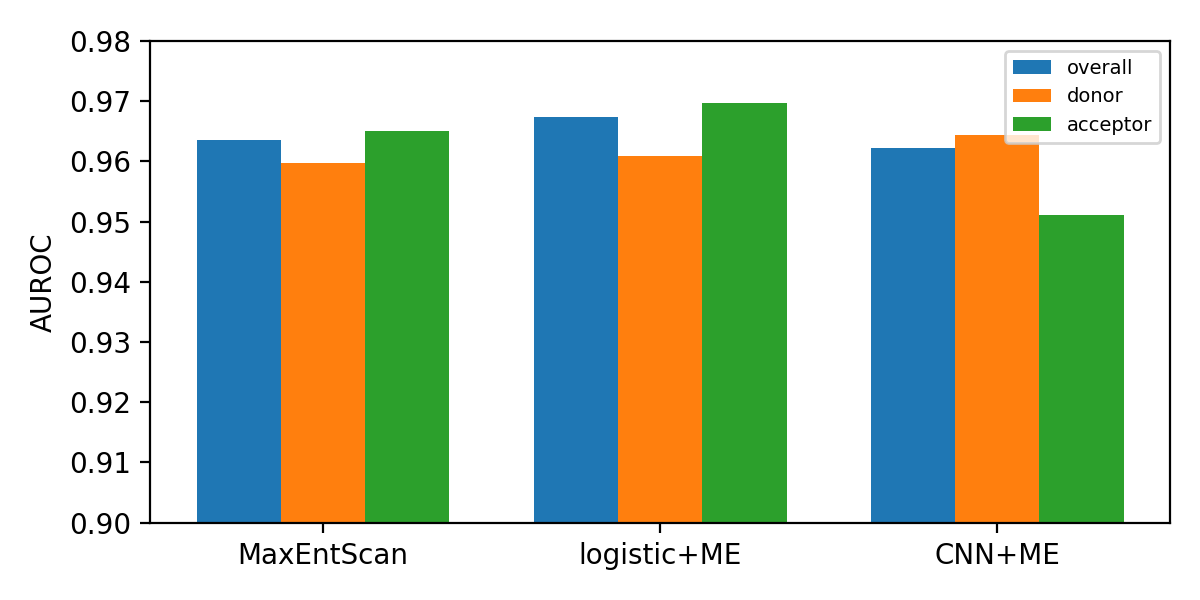
\includegraphics[width=0.85\textwidth]{figs/splice_models.png}\caption{AUROC by model and site type, gene-grouped 5-fold CV.}\end{figure}
\section{Codon Track II: Cross-Species Test of the Ribosomal Reference Set}
Question: Does a ribosomal-protein reference set (Sharp \& Li 1987) make CAI track measured protein abundance better than a genome-wide codon table? Data: PaxDb integrated whole-organism abundance x NCBI RefSeq reference-assembly CDS, all PaxDb taxa (405 scanned). Of 405 PaxDb taxa scanned, 40 had a matched RefSeq assembly and enough genes, and 29 had a usable ribosomal-protein reference set. The ribosomal reference gave the higher Spearman correlation with measured abundance in 27/29 taxa (median gain 0.082; Wilcoxon signed-rank $p=3.3e-07$, sign test $p=1.6e-06$). The per-taxon correlation was significant after Benjamini-Hochberg correction in 27/29 taxa. Exceptions: Rattus norvegicus, Plasmodium falciparum 3D7. The idea goes back to Sharp and Li \cite{sharpli1987}; what is new here is the systematic multi-taxon test with a pre-stated falsification criterion (the claim fails if the ribosomal reference is not better in a majority of taxa at $p<0.01$).
\begin{figure}[h]\centering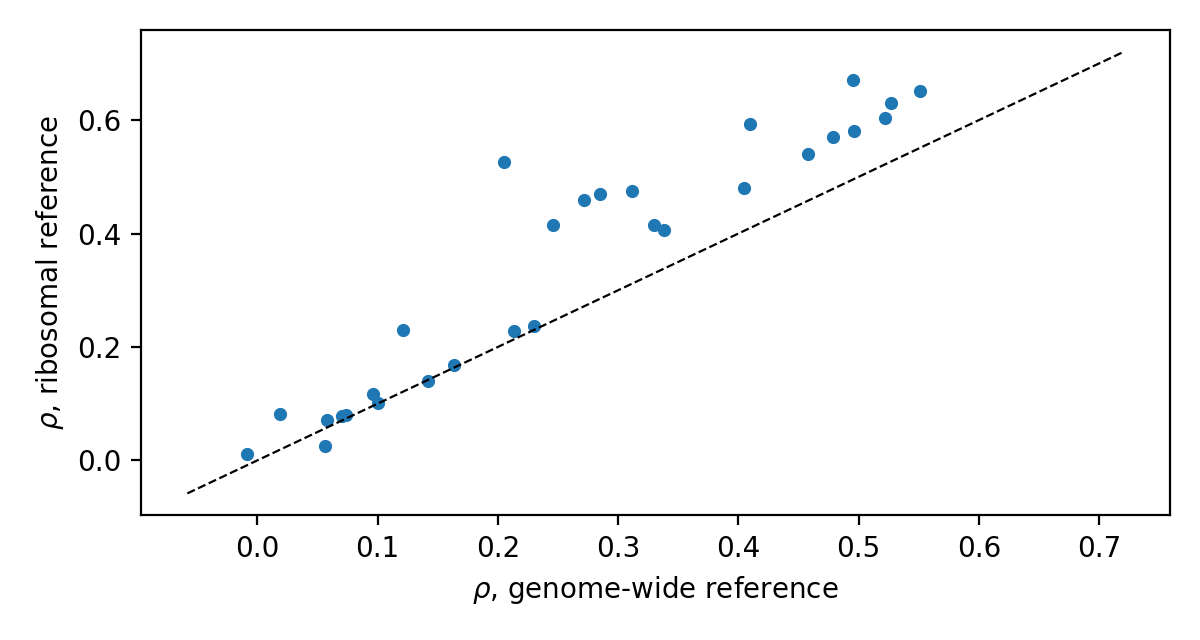
\includegraphics[width=0.9\textwidth]{figs/cai_species.png}\caption{Spearman $\rho$ (CAI vs PaxDb abundance) with the genome-wide versus ribosomal reference, per taxon.}\end{figure}
{\scriptsize\begin{longtable}{lp{4.3cm}lrrrrr}\caption{Per-taxon results (all taxa with a matched assembly).}\\\hline Taxid & Organism & Assembly & $n$ & $n_{ribo}$ & $\rho_{gen}$ & $\rho_{ribo}$ & $q$\\\hline\endhead
10090 & Mus musculus & GCF\_000001635.27 & 8089 & 99 & 0.0704 & 0.0775 & $<$1e-6\\
10116 & Rattus norvegicus & GCF\_036323735.1 & 890 & 124 & 0.142 & 0.1405 & 3.1e-05\\
121845 & Diaphorina citri & GCF\_000475195.1 & 592 & 1 & 0.1458 & -- & --\\
1295 & Staphylococcus schleiferi & GCF\_025558325.1 & 442 & 66 & 0.4583 & 0.5403 & $<$1e-6\\
1314 & Streptococcus pyogenes & GCF\_900475035.1 & 306 & 66 & 0.4954 & 0.6701 & $<$1e-6\\
185431 & Trypanosoma brucei brucei TREU927 & GCF\_000002445.2 & 6302 & 0 & 0.3167 & -- & --\\
192222 & Campylobacter jejuni subsp. jejuni NCTC 11168 = ATCC 700819 & GCF\_000009085.1 & 725 & 66 & 0.1208 & 0.2291 & $<$1e-6\\
196627 & Corynebacterium glutamicum ATCC 13032 & GCF\_000011325.1 & 323 & 72 & 0.5268 & 0.6307 & $<$1e-6\\
198214 & Shigella flexneri 2a str. 301 & GCF\_000006925.2 & 1887 & 72 & 0.5511 & 0.6514 & $<$1e-6\\
208964 & Pseudomonas aeruginosa PAO1 & GCF\_000006765.1 & 4796 & 72 & 0.2459 & 0.4149 & $<$1e-6\\
224308 & Bacillus subtilis subsp. subtilis str. 168 & GCF\_000009045.1 & 3147 & 64 & 0.3295 & 0.4156 & $<$1e-6\\
224911 & Bradyrhizobium diazoefficiens USDA 110 & GCF\_001642675.1 & 494 & 72 & 0.4049 & 0.4806 & $<$1e-6\\
243159 & Acidithiobacillus ferrooxidans ATCC 23270 & GCF\_000021485.1 & 419 & 68 & 0.3378 & 0.4055 & $<$1e-6\\
243230 & Deinococcus radiodurans R1 = ATCC 13939 = DSM 20539 & GCF\_020546685.1 & 319 & 66 & 0.4784 & 0.5698 & $<$1e-6\\
246200 & Ruegeria pomeroyi DSS-3 & GCF\_000011965.2 & 395 & 70 & 0.2714 & 0.46 & $<$1e-6\\
2903 & Emiliania huxleyi CCMP1516 & GCF\_000372725.1 & 484 & 4 & 0.4636 & -- & --\\
343509 & Sodalis glossinidius str. 'morsitans' & GCF\_000010085.1 & 748 & 72 & 0.2849 & 0.4703 & $<$1e-6\\
36329 & Plasmodium falciparum 3D7 & GCF\_000002765.6 & 4946 & 62 & 0.056 & 0.0253 & 0.078\\
403677 & Phytophthora infestans T30-4 & GCF\_000142945.1 & 708 & 0 & 0.5278 & -- & --\\
4081 & Solanum lycopersicum & GCF\_036512215.1 & 426 & 4 & -0.1336 & -- & --\\
4097 & Nicotiana tabacum & GCF\_000715075.1 & 9304 & 0 & -0.0837 & -- & --\\
418985 & Tropilaelaps mercedesae & GCA\_002081605.1 & 2213 & 0 & 0.2207 & -- & --\\
44689 & Dictyostelium discoideum AX4 & GCF\_000004695.1 & 3183 & 10 & -0.3039 & -- & --\\
4932 & Saccharomyces cerevisiae S288C & GCF\_000146045.2 & 5587 & 226 & 0.4099 & 0.5924 & $<$1e-6\\
511145 & Escherichia coli str. K-12 substr. MG1655 & GCF\_000005845.2 & 3486 & 72 & 0.4961 & 0.5809 & $<$1e-6\\
54291 & Klebsiella ornithinolytica & GCF\_030505655.1 & 1038 & 72 & 0.2053 & 0.5268 & $<$1e-6\\
6239 & Caenorhabditis elegans & GCF\_000002985.6 & 11571 & 0 & 0.0748 & -- & --\\
7227 & Drosophila melanogaster & GCF\_000001215.4 & 2251 & 150 & 0.0189 & 0.0813 & 0.00013\\
7460 & Apis mellifera & GCF\_003254395.2 & 879 & 4 & -0.0468 & -- & --\\
8030 & Salmo salar & GCF\_965601325.2 & 1779 & 0 & 0.1332 & -- & --\\
83332 & Mycobacterium tuberculosis H37Rv & GCF\_000195955.2 & 3258 & 76 & 0.2304 & 0.2373 & $<$1e-6\\
9031 & Gallus gallus & GCF\_016699485.2 & 1891 & 68 & 0.2134 & 0.2274 & $<$1e-6\\
93061 & Staphylococcus aureus subsp. aureus NCTC 8325 & GCF\_000013425.1 & 1699 & 58 & 0.5221 & 0.6046 & $<$1e-6\\
9544 & Macaca mulatta & GCF\_049350105.2 & 3732 & 84 & 0.0736 & 0.0808 & 1e-06\\
9606 & Homo sapiens & GCF\_000001405.40 & 12343 & 86 & -0.0083 & 0.0106 & 0.24\\
9615 & Canis lupus familiaris & GCF\_011100685.1 & 329 & 81 & 0.1639 & 0.1673 & 0.0025\\
9823 & Sus scrofa & GCF\_054392235.1 & 3010 & 84 & 0.0576 & 0.071 & 0.00011\\
9913 & Bos taurus & GCF\_002263795.3 & 2694 & 81 & 0.0963 & 0.1177 & $<$1e-6\\
99287 & Salmonella enterica subsp. enterica serovar Typhimurium str. LT2 & GCF\_000006945.2 & 2472 & 72 & 0.3119 & 0.4743 & $<$1e-6\\
9986 & Oryctolagus cuniculus & GCF\_964237555.1 & 1993 & 82 & 0.0999 & 0.1012 & 7e-06\\
\hline\end{longtable}}
$q$ values are stored rounded to 6 decimals; $<$1e-6 marks values that round to zero.
\subsection{tRNA adaptation index and effective number of codons}
Tools: codon-bias (TrnaAdaptationIndex dos Reis s-values, EffectiveNumberOfCodons), GtRNAdb tRNA gene copy numbers. Table~\ref{tab:tai} gives Spearman $\rho$ with abundance. No single index wins everywhere: tAI leads in yeast, the ribosomal-reference CAI leads in \textit{E. coli}, and $-$ENC is weakest in all three organisms.
\begin{table}[h]\centering\small\caption{Codon indices vs abundance (Spearman $\rho$).}\label{tab:tai}\begin{tabular}{p{5cm}rrrrr}\hline Organism & $n$ & CAI$_{gen}$ & CAI$_{ribo}$ & tAI & $-$ENC\\\hline
Escherichia coli str. K-12 substr. MG1655 & 3450 & 0.4961 & 0.5809 & 0.5277 & 0.3836\\
Bacillus subtilis subsp. subtilis str. 168 & 3115 & 0.3295 & 0.4156 & 0.4146 & 0.1735\\
Saccharomyces cerevisiae S288C & 5474 & 0.4099 & 0.5924 & 0.6604 & 0.4471\\
\hline\end{tabular}\end{table}
\section{Docking Track: Real AutoDock Vina Against LP-PDBBind}
Source: LP-PDBBind (github.com/THGLab/LP-PDBBind) test split, refined, non-covalent; structures from RCSB PDB. Engine: AutoDock Vina 1.2.7 (exhaustiveness 8, 24 A box on crystal ligand) + Open Babel 3.1.1 prep, pH 7.4. 73/80 complexes ran; the 7 failures are listed in Table~\ref{tab:dockerr}. Redocking: top-1 pose RMSD $<2$\,\AA{} in 52.0\% and best-of-9 in 83.6\% (RMSD without symmetry correction (conservative)). Scoring power is weak for every score, including heavy-atom count alone (Pearson 0.2445): Vina top pose 0.2854 (95\% CI [0.055, 0.485]), sugarcode's own Vina-like score on the crystal pose 0.2975 (CI [0.027, 0.484]). The honest reading: sugarcode's scoring term adds nothing beyond ligand size on this split, so the module now calls real Vina (sugarcode-ai commit e0564e4) instead of claiming affinity prediction.
\begin{figure}[h]\centering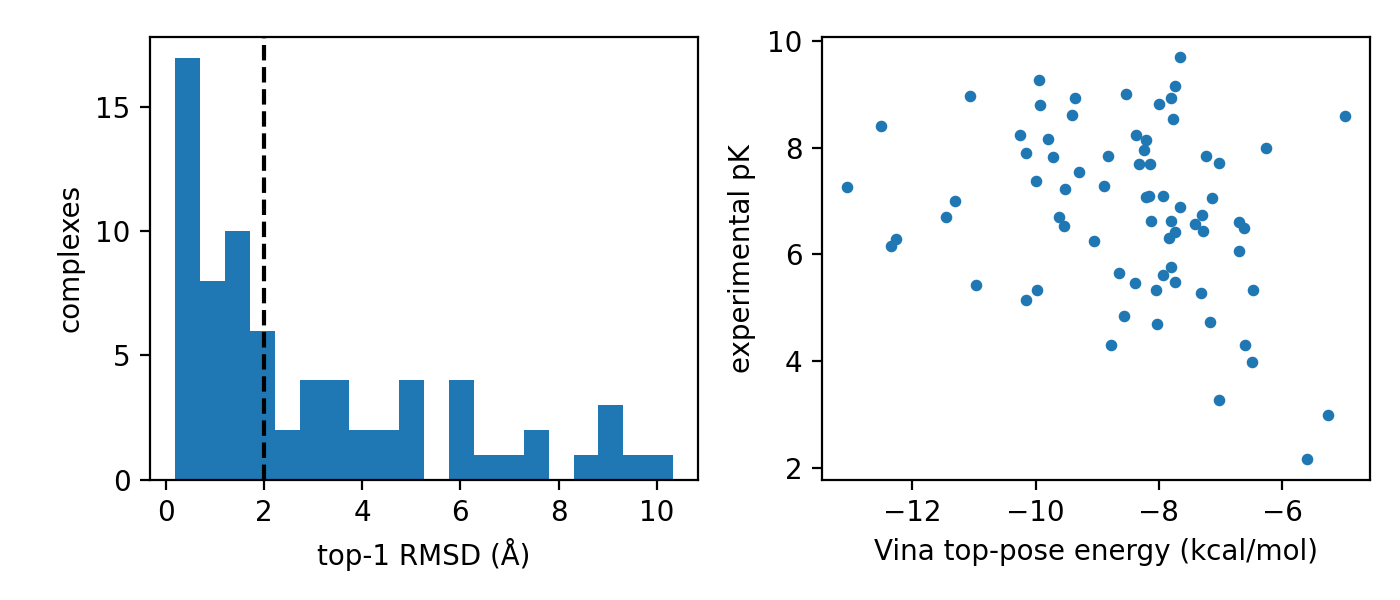
\includegraphics[width=0.9\textwidth]{figs/docking.png}\caption{Left: redocking RMSD distribution. Right: Vina top-pose energy vs experimental pK.}\end{figure}
\begin{table}[h]\centering\small\caption{Docking failures.}\label{tab:dockerr}\begin{tabular}{ll}\hline PDB & Error\\\hline
4cws & no ligand match\\
4q08 & no ligand match\\
3hkt & no ligand match\\
4r74 & no ligand match\\
3p4v & no ligand match\\
4ou3 & no ligand match\\
5ep7 & no ligand match\\
\hline\end{tabular}\end{table}
{\scriptsize\begin{longtable}{lrrrrrrr}\caption{Per-complex docking results.}\\\hline PDB & pK & heavy & $E_{cryst}$ & $E_{min}$ & $E_{top}$ & RMSD$_1$ & RMSD$_{9}$\\\hline\endhead
1cnw & 7.72 & 26 & -4.19 & -5.37 & -7.02 & 7.26 & 6.03\\
1o3l & 6.54 & 24 & -7.09 & -8.63 & -9.54 & 3.19 & 1.09\\
3po6 & 7.06 & 19 & -4.54 & -6.13 & -7.14 & 3.81 & 0.86\\
4db7 & 6.56 & 18 & -6.63 & -7.18 & -7.41 & 0.52 & 0.52\\
5sz5 & 7.7 & 17 & -7.33 & -7.33 & -8.14 & 0.39 & 0.39\\
4mo8 & 8.0 & 16 & -4.75 & -5.50 & -6.25 & 2.29 & 1.52\\
4tim & 2.16 & 11 & -3.41 & -4.13 & -5.59 & 1.66 & 1.66\\
1ejn & 5.62 & 25 & -8.20 & -8.43 & -7.93 & 2.51 & 2.15\\
5d3l & 6.06 & 30 & -6.22 & -6.32 & -6.70 & 8.34 & 1.64\\
3b3c & 3.98 & 10 & -5.07 & -5.76 & -6.48 & 1.42 & 1.42\\
3r4n & 6.89 & 23 & -6.79 & -7.37 & -7.66 & 0.81 & 0.81\\
2p4j & 8.96 & 49 & -10.13 & -10.73 & -11.07 & 1.58 & 1.58\\
5sz4 & 9.7 & 16 & -7.04 & -7.33 & -7.65 & 1.79 & 1.79\\
4xit & 7.27 & 32 & -12.19 & -12.80 & -13.06 & 0.96 & 0.96\\
5mjn & 8.54 & 18 & -6.42 & -6.93 & -7.76 & 5.97 & 1.41\\
2xjg & 7.82 & 23 & -9.04 & -9.53 & -9.72 & 0.25 & 0.25\\
5ix0 & 6.28 & 25 & -11.86 & -12.14 & -12.27 & 0.27 & 0.27\\
5y8y & 7.09 & 25 & -6.08 & -6.38 & -8.16 & 4.75 & 0.84\\
6g38 & 6.62 & 19 & -7.36 & -7.70 & -8.12 & 0.61 & 0.61\\
4o04 & 6.16 & 26 & -11.03 & -12.14 & -12.36 & 1.34 & 1.34\\
5ewk & 4.85 & 22 & -7.91 & -7.96 & -8.57 & 0.68 & 0.68\\
3d8w & 8.15 & 19 & -6.96 & -7.48 & -8.20 & 1.43 & 1.43\\
4rfc & 8.24 & 23 & -5.25 & -6.44 & -8.37 & 7.44 & 5.67\\
3r17 & 6.41 & 20 & -6.73 & -7.38 & -7.74 & 3.57 & 2.30\\
4knj & 7.95 & 21 & -6.40 & -7.32 & -8.23 & 4.81 & 1.87\\
6g6t & 7.7 & 19 & -7.42 & -7.76 & -8.31 & 2.10 & 0.61\\
4lxz & 6.74 & 19 & -6.37 & -6.47 & -7.29 & 6.21 & 1.95\\
5o87 & 6.61 & 12 & -5.46 & -6.58 & -6.70 & 0.44 & 0.44\\
4j93 & 4.7 & 21 & -7.50 & -7.81 & -8.02 & 0.44 & 0.44\\
6hrq & 7.09 & 23 & -6.44 & -6.94 & -7.94 & 6.23 & 2.21\\
4nh7 & 8.4 & 33 & -11.46 & -12.05 & -12.52 & 1.31 & 1.31\\
2x7t & 6.63 & 30 & -6.30 & -7.34 & -7.81 & 6.16 & 0.77\\
4fl1 & 3.28 & 31 & -5.80 & -5.98 & -7.02 & 9.18 & 2.47\\
3c84 & 7.85 & 16 & -6.59 & -6.98 & -7.23 & 0.39 & 0.39\\
4ytc & 7.89 & 26 & -9.65 & -10.13 & -10.15 & 0.49 & 0.49\\
2zdn & 6.25 & 27 & -7.86 & -8.84 & -9.05 & 1.02 & 1.02\\
5f60 & 7.37 & 37 & -8.55 & -8.90 & -9.99 & 4.69 & 1.63\\
6hqy & 6.44 & 22 & -5.86 & -6.97 & -7.28 & 2.03 & 1.48\\
5l8c & 7.0 & 35 & -8.93 & -9.64 & -11.31 & 9.53 & 0.86\\
1p1o & 5.76 & 13 & -7.26 & -7.37 & -7.79 & 0.60 & 0.60\\
5htz & 8.62 & 26 & -9.05 & -9.25 & -9.40 & 0.19 & 0.19\\
4oag & 6.3 & 27 & -5.33 & -7.22 & -7.84 & 9.16 & 3.85\\
2j4i & 9.0 & 36 & -8.00 & -8.56 & -8.54 & 1.38 & 1.38\\
5n24 & 8.92 & 18 & -7.04 & -7.44 & -7.80 & 1.68 & 1.40\\
1y3x & 5.14 & 33 & -9.50 & -9.83 & -10.15 & 0.70 & 0.70\\
1f5l & 5.28 & 15 & -6.27 & -7.20 & -7.32 & 2.87 & 1.51\\
5aml & 9.15 & 21 & -6.79 & -6.99 & -7.74 & 5.22 & 1.14\\
6u6w & 5.33 & 21 & -7.71 & -7.69 & -8.04 & 5.13 & 0.33\\
5mpn & 7.07 & 23 & -6.86 & -7.18 & -8.21 & 7.46 & 1.25\\
4jfm & 5.48 & 35 & -6.54 & -7.29 & -7.74 & 0.97 & 0.97\\
5ewy & 4.3 & 22 & -7.30 & -7.87 & -8.78 & 3.50 & 2.90\\
4zme & 4.3 & 19 & -6.04 & -6.27 & -6.60 & 10.33 & 0.18\\
4yxi & 6.5 & 11 & -5.93 & -6.43 & -6.62 & 0.39 & 0.39\\
2erz & 5.66 & 21 & -7.23 & -8.31 & -8.65 & 2.99 & 0.93\\
6oe0 & 8.92 & 27 & -7.95 & -8.86 & -9.35 & 0.86 & 0.86\\
4b2i & 3.0 & 9 & -4.33 & -5.04 & -5.25 & 1.97 & 0.61\\
4f5y & 5.43 & 46 & -10.70 & -11.84 & -10.97 & 3.66 & 3.66\\
6eq5 & 4.74 & 10 & -6.31 & -6.71 & -7.17 & 2.09 & 0.51\\
5g5v & 6.7 & 36 & -10.54 & -10.73 & -11.46 & 2.75 & 1.52\\
5cau & 8.8 & 34 & -9.64 & -9.84 & -9.93 & 0.65 & 0.65\\
1gi1 & 5.47 & 19 & -6.60 & -8.25 & -8.38 & 0.77 & 0.77\\
3hkq & 5.34 & 15 & -4.38 & -5.42 & -6.47 & 3.67 & 3.04\\
2xab & 9.27 & 22 & -9.46 & -9.81 & -9.94 & 0.21 & 0.21\\
3hll & 8.24 & 30 & -9.62 & -10.25 & -10.25 & 0.36 & 0.36\\
5f62 & 8.17 & 38 & -8.66 & -9.01 & -9.80 & 4.22 & 1.46\\
3ibi & 8.59 & 13 & -4.21 & -4.73 & -4.97 & 5.02 & 3.28\\
3m35 & 7.22 & 37 & -8.52 & -9.07 & -9.52 & 0.90 & 0.90\\
1g54 & 8.82 & 25 & -7.03 & -7.63 & -8.00 & 8.95 & 8.89\\
4r76 & 7.85 & 26 & -7.58 & -8.26 & -8.82 & 1.62 & 1.62\\
1zgi & 5.34 & 32 & -9.23 & -9.64 & -9.98 & 0.76 & 0.76\\
5cap & 7.28 & 29 & -8.09 & -8.54 & -8.89 & 1.44 & 1.44\\
1k1j & 7.55 & 37 & -8.36 & -8.62 & -9.29 & 1.77 & 1.77\\
6rfn & 6.7 & 35 & -7.10 & -8.72 & -9.63 & 6.69 & 1.10\\
\hline\end{longtable}}
